\documentclass{article}
\usepackage{parskip}
\usepackage{graphicx}
\usepackage[margin=.6in]{geometry}

\begin{document}
\section*{Interpretor} % (fold)
\label{sec:interpretor}
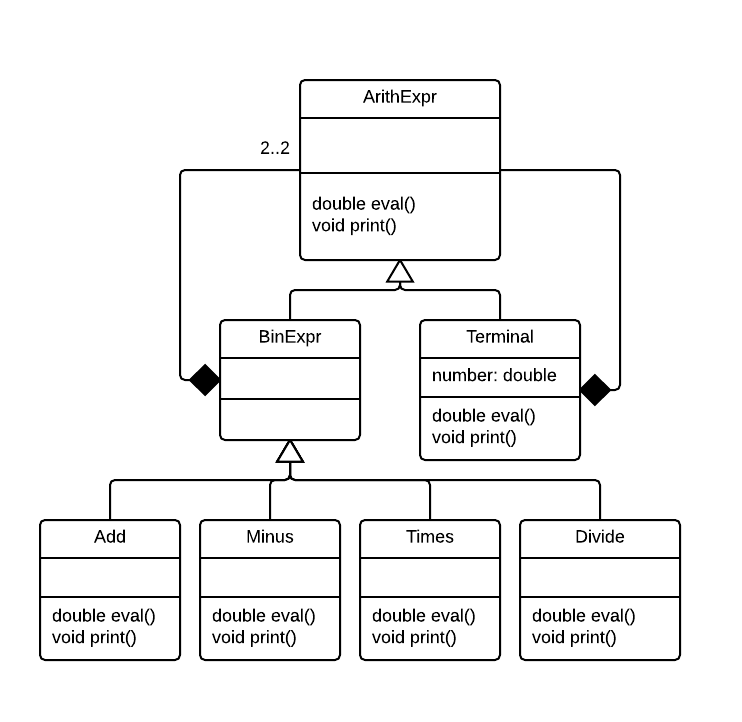
\includegraphics[width=7in]{interpretor.png}

The interpretor pattern builds a recursive structure of expressions and their sub expressions and calls its own eval function by calling the eval function of its children expression and then conducting its operation on the results.
% section interpretor (end)

\newpage
\section*{Visitor} % (fold)
\label{sec:visitor}
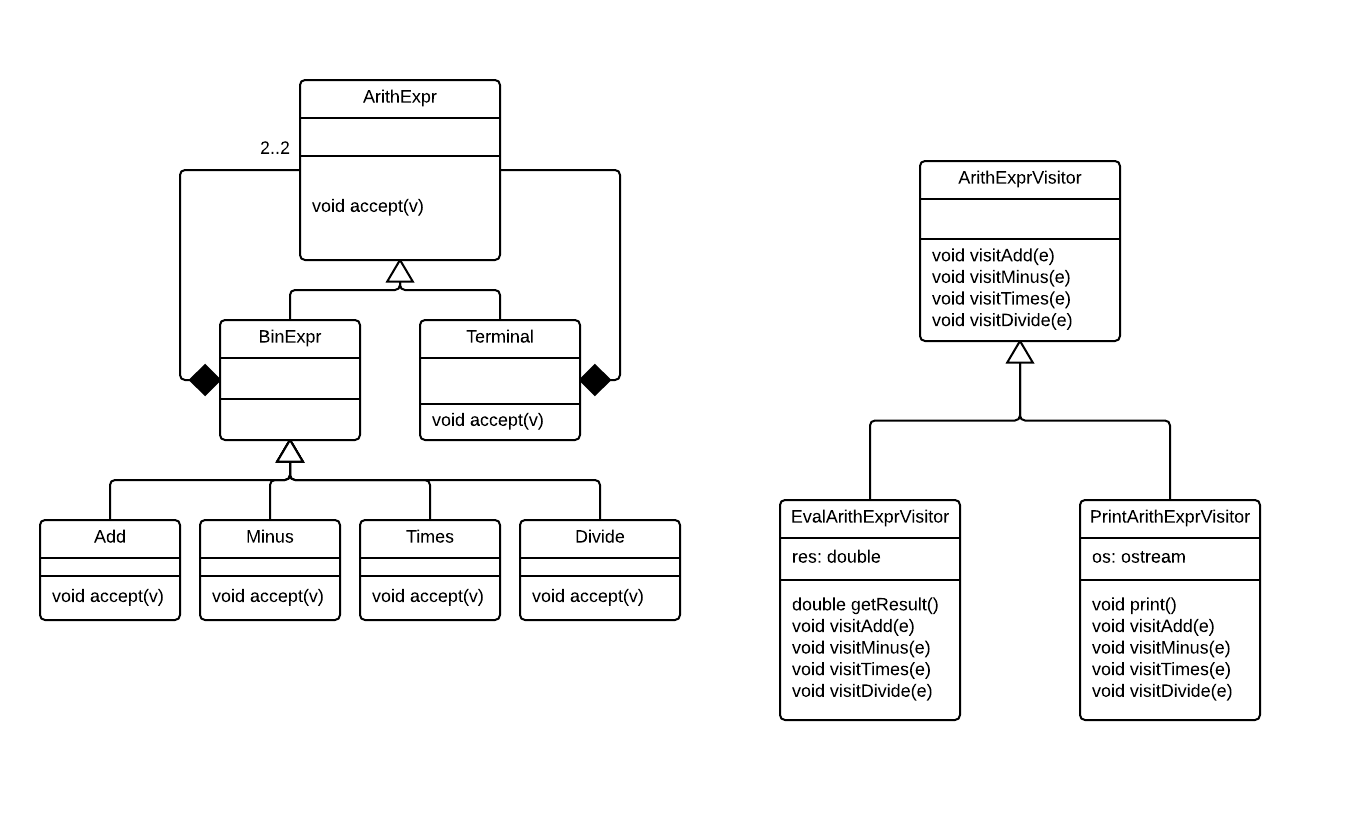
\includegraphics[width=7in]{visitor.png}

The visitor pattern builds a similar parsing structure as the interpretor pattern. then creates a hierarchy of visitors that ``visit'' objects in that parsing tree and preform actions on them.
% section visitor (end)

\newpage
\section*{Out of the Box} % (fold)
\label{sec:box}
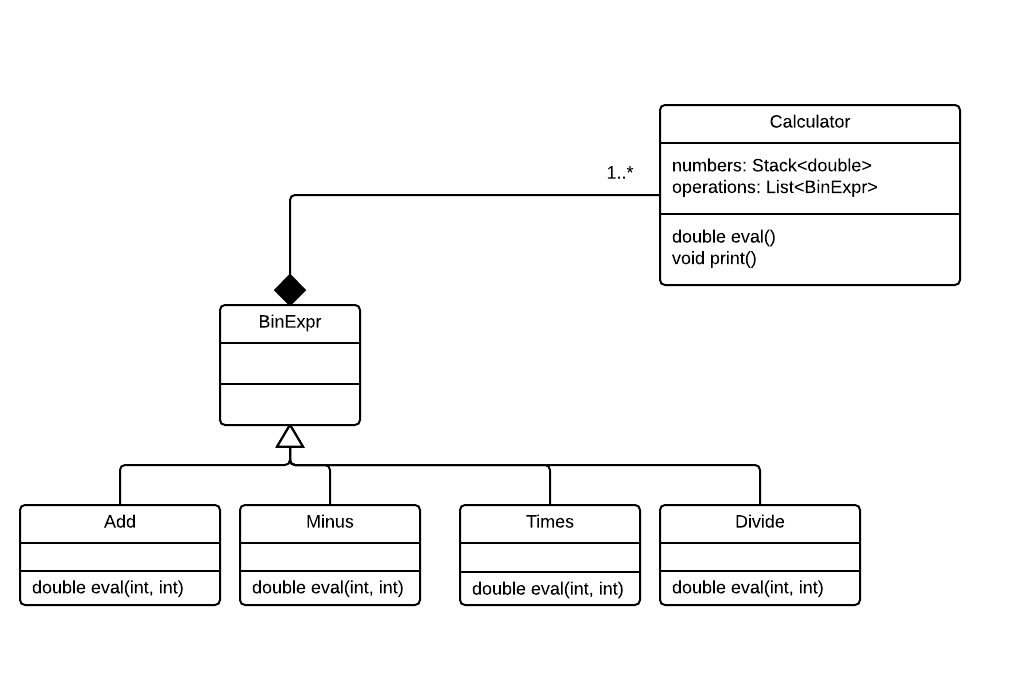
\includegraphics[width=7in]{rpn.png}

When the RPN string is read in it can be parsed into a stack of numbers (in reverse order by pushing on to the top as you read) and an list of operations to be preformed in order. The operations are of type BinExpr class which has subclasses for each function with their own eval function that takes two numbers. When the Calculator class' eval function is called it iterates through its operations popping numbers off of its stack and evaluating as it goes. It uses a BinExpr class to group all operations as subclasses allowing a single list of operations to exist. Each operation has a eval operation to do the correct mathematical operation.
% section box (end)

\newpage
\section*{Cheating} % (fold)
\label{sec:cheating}
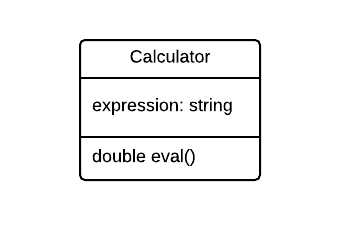
\includegraphics{cheat.png}

This is Calculator class is just a Jython class that use python's built in eval function to just return the evaluation of the string with no other parsing required. It just takes in the string to be evaluated and does no parsing on it.

% section cheating (end)
\newpage

\section*{Analysis} % (fold)
\label{sec:analysis}
\subsection*{Fitness for Purpose} % (fold)
\label{sub:fitness_for_purpose}
All of the above designs support evaluation of arithmetic expressions.
% subsection fitness_for_purpose (end)
\subsection*{Production Costs} % (fold)
\label{sub:production_costs}
The interpretor pattern requires 7 classes, visitor pattern requires 10 classes, out of the box pattern requires 6 classes, and the cheating pattern requires one class. By basic cost analysis the cheating pattern requires knowledge of Jython and the interpretor and visitor patterns require knowledge of how they work to implement. Roughly speaking the cheating pattern requires the least amount of work to implement followed by the out of the box pattern. The interpretor pattern is slightly easier than the visitor since it doesn't require the implementation of the visitor classes.
% subsection production_costs (end)
\subsection*{Fitness for Future} % (fold)
\label{sub:fitness_for_future}
The interpretor pattern, and visitor pattern could add the factorial function by adding a unary expression subclass off of the arithmetic expression class and giving that class a factorial subclass to allow iterations to still be parse properly and evaluate correctly. The out of the box pattern could easily add a factorial function by adding another subclass for it on the BinExpr class. The cheating pattern could support factorials without adding a new subclass since the factorial function is supported by python's eval function.

The interpretor pattern can add a pretty print functionality by adding print functions to each operation and terminals. This function is called on expressions recursively so that it prints bounding brackets then its self. The visitor pattern can add printer functionality by adding a visitor that prints as its function. The out of the box design pattern can add pretty print functionality by adding  a print function on the calculator class and operator classes. This will work similar to the printer functionality for the interpretor pattern. The cheating design pattern cannot support pretty printing easily as it does no parsing of the string it gets. A whole new parser will be required to add this functionality.


\subsection*{Design Structure} % (fold)
\label{sub:design_structure}
The visitor and interpretor patterns both use the composite pattern to parse large complex expressions into smaller expressions. This allows the interpretor and visitor patterns to treat large expressions as if they were simple expressions or terminals. This allows those patterns to apply simpler functions to them and let it recurse through the function. It also means that we can extend the pattern to handle different types of expressions or increase their complexity by simply adding more subclasses to the composite portion of the design without altering how things interact.
% subsection design_structure (end)
% subsection fitness_for_future (end)





% section analysis (end)
\end{document}
